\documentclass{scrartcl}

\usepackage[utf8]{inputenc}
\usepackage[T1]{fontenc}
\usepackage[ngerman]{babel}
\usepackage{fancyhdr}
\usepackage{listings}
\usepackage{csquotes}
\usepackage{tikz}
\usepackage{algorithm2e}
\usepackage{float}

\usepackage{lscape}

\usetikzlibrary{automata,positioning}

\title{Verteiltes Genom Browsing}
\subtitle{Projektspezifikation}
\date{1. Dezember 2015}
\setkomafont{subtitle}{\bfseries \LARGE}
\renewcommand{\headrulewidth}{0pt}
\date{23. Dezember 2015}


\newcommand{\includepicture}[3][width=\textwidth] {
\begin{figure}[H]
  \centering
	\includegraphics[#1]{#2} 
  \caption{#3}
  \label{fig:#3}
\end{figure}
\hfill\\
}
\begin{document}
\pagestyle{fancy}
%\fancyhf{}
\cfoot{}
\rfoot{\pagemark}
\lhead{}
\rhead{}


\setcounter{page}{-2}
\maketitle
\thispagestyle{empty}
\newpage
\thispagestyle{empty}
\tableofcontents
\thispagestyle{empty}
\newpage
%\section{Einleitung}
%\newpage
% !TEX root = Projektspezifikation.tex
\section{Einleitung}
Dieses Dokument ist die Projektspezifikation für das Semesterprojekt zur verteilten Echtzeitrecherche in Genomdaten. 
Hierbei umfasst der Begriff "'Genomdaten"':
\\
\begin{description}
\item[Chromosomen] enthalten das Erbgut eines Menschen. Sie enthalten somit die DNA, auf welcher die einzelnen Gene abgebildet sind. Verschiedene Spezies haben unterschiedlich viele Chromosomen und Gene. 
\\ Für dieses Projekt beziehen wir uns ausschließlich auf die 24 Chromosomen des Menschen. Hier sind die zwei Geschlechtschromosomen X und Y bereits enthalten.

\item[Gene] bestehen aus einer Sequenz von Basen, welche ein zu synthetisierendes Protein kodieren. Jedes Gen kodiert ein oder mehrere Proteine. Jedes Gen kann auf Grund seiner Genkoordinaten entweder identifiziert, oder seine Sequenz anhand der Koordinaten gefunden werden.

\item[Genkoordinaten] geben an, auf welchem Abschnitt von welchem Chromosom ein Gen liegt. Chromosom und Gen bilden somit die Koordinate.
Hierbei werden die untere und die obere Grenze angegeben.

\item[Basenpaare] ergeben sich durch die Doppelhelix-Struktur der DNA.\\ Es gibt vier Basen:
\begin{enumerate}
\item Adenin (A) 
\item Cytosin (C)
\item Guanin (G)
\item Thymin (T)
\end{enumerate}
 von denen jeweils zwei Gegenstücke zueinander sind. Diese Paare sind A - T und C - G. Es folgt also, dass nur diese Basenpaare in der Helix vorhanden sind.\\
Spricht man von Mbp, so sind dies Megabasenpaare, hierbei entspricht\\
1Mbp = 1000000 Bp (Basenpaare).

\item[Mutationen] sind Abweichungen in der Basensequenz eines Gens zum Referenzgenom. Das heißt:\\Unterscheidet sich an einer spezifischen Stelle des Chromosoms eines Probanden eine Base zu der im Referenzgenom verzeichneten, so kann dies eine Punktmutation sein. Wirkt sich die Veränderung jedoch nicht weiter aus, so handelt es sich nur um eine Variante des Basenpaares. Dies wird auch als Einzelnukleotid-Polymorphismus (SNP) bezeichnet.\\
Weiterhin existieren bestimmte Basensequenzen innerhalb der Gen, welche mehrfach hintereinander wiederholt werden. Die Anzahl der Wiederholungen kann von Mensch zu Mensch unterschiedlich sein. Diesen Sachverhalt bezeichnet man als Kopienzahlvariation (CNV).\\
Neben CNVs können auch fehlende oder zusätzliche Basenpaare in bestimmten Basensequenzen auftreten. Diese fehlenden bzw. zusätzlichen Basenpaare bezeichnet man als Indel.\\


\item[Das Referenzgenom] wird in unregelmäßigen Abständen neu ermittelt. Anhand dieses Genoms werden alle weiteren Sequenzierungen von Basenpaaren überprüft und Mutationen ermittelt. Das aktuelle Referenzgenom GRCh38.p5\footnote{\label{foot:0}http://www.ncbi.nlm.nih.gov/projects/genome/assembly/grc/human/} ist am 25. September 2015 herausgegeben worden.
\end{description}
Im folgenden Dokument wird die Realisierung des Softwareprojektes erläutert.
\newpage


\section{Aufgabenstellung und Anforderungen}
\subsection{Aufgabenstellung}
Es soll ein System entwickelt werden, welches in Echtzeit Genomdaten durchsucht und die grafische Auswertung übernimmt. 
\subsection{Anforderungen}
\begin{itemize}

\item Es werden vier Datenbanken fest integriert: 
\begin{itemize}
\item HGMD\footnote{\label{foot:1}http://www.hgmd.cf.ac.uk/ac/index.php}
\item dbSNP\footnote{\label{foot:2}http://www.ncbi.nlm.nih.gov/SNP/}
\item 1000 Genomes Project\footnote{\label{foot:3}http://www.1000genomes.org/}
\item The Cancer Genome Atlas: Lung and Colorectal Cancer\footnote{\label{foot:4}http://cancergenome.nih.gov/}
\end{itemize}
Weiterhin wird das System für weitere (eigene) Datenquellen erweiterbar sein.

\item Folgende Informationen werden bereitgestellt:
\begin{itemize}
\item Metadaten: Datenquelle, Zeitpunkt des Downloads
\item Genkoordinate der Mutation (ggf. Abschnitt)
\item Mutierte Basensequenz (auch Referenzgenom muss bekannt sein)
\item (relative) Häufigkeit der Mutationen
\item Quellspezifische Sample-Attribute (Krankheit, Geschlecht, etc.)
\end{itemize}

\item Eine Anfrage wird in <1 Sekunde durchlaufen.\\
Zulässige Anfragen sind:
\begin{itemize}
\item Intervallanfragen:
\begin{itemize}
\item Anfrage mit: Chromosom, linke und rechte Grenze (Genkoordinaten)
\item Systemkorrektur: Intervall >10Mbp führt dazu, dass ein Fehler geworfen wird
\item Ergebnis: Mutationen in dem Abschnitt
\end{itemize}
\item Genanfragen:
\begin{itemize}
\item Anfrage mit: Name eines humanen Gens
\item Systemkorrektur: Namensvorschläge, wenn Genname nicht vollständig bekannt
\item Ergebnis: Vom System bestimmter Genabschnitt, sowie die darauf befindlichen Mutationen
\end{itemize} 
\end{itemize}
\newpage
Folgende Filter werden zur Suchoptimierung angeboten:
\begin{itemize}
\item Einschänkung auf Quelle
\item Einschänkung auf relative Häufigkeit
\item Gleichheit quellspezifischer Attribute
\end{itemize}

\item Die Darstellung erfolgt:
\begin{itemize}
\item je Datenquelle
\item mit einem max. 10Mbp großen Ausschnitt des Chromosoms
\item mit Referenzgenom zum Vergleich bei kleinen Abschnitten
\item mit Anzeige der Basenpaare und Markierung von Mutationen in kleinen Abschnitten ($\leq$ 200Bp)
\item mit Andeutung der Verteilung der Häufigkeit von Mutationen in großen Abschnitten (> 200Bp)
\end{itemize}
Zudem bietet das Interface interaktive Möglichkeiten:
\begin{itemize}
\item Zoomfunktion mit fünf Stufen, um den dargestellten Bereich zu verkleinern oder zu vergrößern
\item Scrollen, um sich horizontal auf dem Chromosom fortzubewegen
\item Konfigurationsmöglichkeiten zur Darstellung und anderer Systembereiche
\end{itemize}

\item Das System wird unter Mozilla Firefox laufen und auf bestehenden Webservern leicht einzurichten sein
\end{itemize}

\newpage
\section{Beispiele zur Nutzung: Use Cases}
\subsection{Use Case 1}
Ein Benutzer möchte herausfinden, welche Mutationen im Bereich von 144MB – 154MB auf dem Chromosom 7 auftreten können. Hierfür wählt er die 1000 Genomes Projekt-Datenbank aus. \\
Das ganze Chromosom wird in einem eigenen Anzeigebereich (Lane) im Vergleich zum Referenzgenom angezeigt. Er erkennt durch eine Markierung, dass im Bereich von 150MB-152MB gehäuft Mutationen auftreten können. Da er diesen Bereich nicht detailliert einsehen kann, zoomt der Benutzer herein. Die Basenpaare in der 1000 Genomes-Lane sind immer detaillierter zu erkennen, bis er genau einsehen kann, welche Mutationen auftreten können. Bei Erreichen der maximale Zoomstufe, sind alle Basenpaare des Chromosoms 7 und des Referenzgenoms, das nun eingeblendet wird, zu erkennen und er kann die auftretenden Mutationen betrachten.
\subsection{Use Case 2}
Ein Benutzer möchte herausfinden, welche Mutationen bei einer bestimmten relativen Häufigkeit im Bereich eines Gens auftreten. Da er sich sehr für den colorectalen Bereich interessiert, wählt er The Cancer Genome Atlas (TCGA) aus. Da der Benutzer nicht den genauen Namen des Gens kennt und sich bei der Eingabe irrt, bekommt er keine Basenpaare angezeigt, sondern Vorschläge, welches Gen er gesucht haben könnte. Auf Grund der Vorschläge erinnert sich der Benutzer und wählt das korrekte Gen. \\
Es erscheint eine Lane, welche die Daten für den Bereich darstellt und der Benutzer erkennt die Bereiche, in welchen Mutationen auftreten. Zusätzlich werden ihm die relativen Häufigkeiten der Mutationen angezeigt.
\subsection{Use Case 3}
Ein Benutzer möchte sich darüber informieren, mit welcher Häufigkeit in einem bestimmten Bereich eines bestimmten Gens Mutationen auftreten können. Hierbei wählt er die HGMD mit einem Bereich von 140MB – 155MB. Da der Bereich jedoch zu groß ist,
wird ihm nur der Bereich von 140MB-150MB dargestellt. \\
Er erkennt in diesem Bereich, dass sehr wenig Mutationen auftreten. Ihn interessiert jedoch ebenfalls, ob bei Krebspatienten höhere Mutationsraten existieren. Dazu führt er die gleiche Suche noch einmal aus, wählt jedoch zusätzlich TCGA für Lungenkrebs und TCGA für Colorectalkrebs. \\
Als Ergebnis werden ihm die drei Lanes untereinander angezeigt und er kann die Häufigkeit von Mutationen in den Bereichen vergleichen.

\newpage
\section{Umsetzung}
\subsection{Vorgehensweise des Systems}
Damit dem System Daten zur Verfügung stehen, müssen die vier Hauptdatenbanken zuerst aus dem Internet heruntergeladen werden.\\
Nachdem der Download erfolgreich war, werden die Datenbanken in ein einheitliches Format überführt. Ist die Vereinheitlichung vollzogen, können nun die humanen Datensätze herausgefiltert und in die eigens entworfene Datenbank (DWH) eingespeichert werden.
\\
Sind alle Daten verarbeitet und somit das DWH vollständig, stehen die Daten bei Programmstart zum Aufbau des verteilten Index zur Verfügung. \\
Wurde der verteilte Index fertig gebaut, kann der Benutzer nun Anfragen an das System absenden. Die Anfragen werden vom Benutzeroberfläche (GUI) an die Middleware geschickt. Hier werden die Anfragen validiert und gegebenenfalls korrigiert. Sind die Anfragen korrekt, werden diese über dem verteilten Index ausgeführt und die Ergebnisse an das GUI zurückgegeben. Hat das GUI die Ergebnisdaten empfangen, werden diese grafisch aufbereitet.\\\\
Folgendes Kommunikationsdiagramm verdeutlicht hierbei den Ablauf:\\\\
\begin{center}
\begin{tikzpicture}[%
>=stealth,
node distance=5cm,
on grid,
draw,
align=left
]
\node[rectangle, draw, initial,initial text=] (0) {Download\\der Datensätze};
\node[rectangle, draw] (1) [right=3cm of 0] {Parsing};
\node[rectangle, draw] (2) [right=3cm of 1] {Einfügen\\in DHW};
\node[rectangle, draw] (3) [below=2cm of 0] {Aufbau der \\Index Bäume};
\node[rectangle, draw] (4) [right of=3] {Suchoperationen in den\\Bäumen ausführen};
\node[rectangle, draw] (5) [below=2cm of 3] {Daten darstellen};
\path[->] (0) edge node {} (1);
\path[->] (1) edge node {} (2);
\path[->] (2) edge node {} (3);
\path[->] (3) edge node {} (4);
\path[<->,bend left, left] (4) edge node {JSON} (5);
\end{tikzpicture}
\end{center}
\newpage
\subsection{Arbeitsbreiche}
Zur Umsetzung des Systems müssen, wie aus \textit{4.1} hervorgeht, drei Hauptbereiche abgedeckt werden. Diese sind:
\begin{description}
\item[Integration:] Zuständigkeitsbereiche der Integration sind die Aufbereitung der Datenquellen und die Bereitstellung der aufbereiteten Datensätze in einer eigens entworfenen Datenbank.

\item[Middleware:] Die Middleware ist für die Kommunikation zwischen Datenbank und Frontend zuständig. Um die vom Frontend an die Middleware gesendeten Anfragen effizient bearbeiten zu können, befasst sich die Middleware mit dem Entwurf eines verteilten Index. Dieser ermöglicht die zeiteffiziente Suche in den Daten der Datenbank und somit eine zeiteffiziente Rückgabe der Ergebnisse an das GUI.

\item[Frontend:] Das Frontend ist für die grafische Aufbereitung der Ergebnisdaten, sowie für das GUI zur Bedienung des Systems zuständig.
\end{description}
Im folgenden werden die Teilbereiche, die Grundzüge ihrer Realisierung, sowie die Verwendung findenden Technologien erläutert. Des Weiteren werden offene Fragen und Risiken der einzelnen Realisierungen angesprochen.
\newpage

% !TEX root = Projektspezifikation.tex

\section{Integration}
\subsection{Integrationsprozess}
\subsubsection{Ablauf der Integration}
Die Software wird standardmäßig zwei Quellen integriert haben: die dbSNP und das 1000GenomeProject. Diese werden, über ein Skript gesteuert, heruntergeladen. Wenn dieser Part abgeschlossen ist, wird ein lokaler Parser (später mehr zu den Parsern und ihrer Arbeitsweise) alle relevanten Daten aus den heruntergeladenen Dateien extrahieren und sie in einem, für den globalen Parser akzeptablen Format bereitstellen. Der globale Parser wird diese Dateien dann in Datensätze staffeln und diese dann in das Data Ware House einfügen um sie dann so der Middleware für die Abfragen bereitzustellen.\\
Der lokale Parser wird benötigt, da es kein allgemeingültiges Standardformat gibt, in dem die Dateien abgespeichert werden. Die Formate sind auch keine, von dem DWH anerkannten, Dateiformate, die integriert werden können. Hinzu kommt, dass Sehr viele weitere Daten, die nicht notwendig sind, in den Dateien vorhanden sind und somit nur die benötigten Daten ausgelesen werden müssen.\\
Wenn der User weitere Quellen integrieren möchte, benötigt er zwei Dinge dafür: Ein Downloadskript, welches von der gewünschten Quelle die Dateien herunterlädt, und ein lokaler Parser, der die heruntergeladenen Dateien danach für den globalen Parser bereitstellt.
\subsubsection{Quellenauswahl}
Die Quellen, die von uns integriert sein werden, werden die dbSNP und das 1000GenomeProject sein, da diese alle benötigten Daten frei zugänglich bereitstellen, ohne jegliche Gegenleistung zu verlangen. HGMD hingegen können wir nicht integrieren, da für die Benutzung ihrer Daten eine Lizenz erworben werden muss, die den finanziellen Rahmen des gesamten Projektes sprengt. TCGA konnten wir bei unserer anfänglichen Quellensichtung als "nicht nutzbar" für das Projekt einstufen, da es weder eine Angabe auf ein Referenzgenom gibt, auf das sich die Daten beziehen, noch gibt es Metadaten für die Mutationen. Sollte sich noch eine Möglichkeit ergeben, die Quelle doch integrieren zu können, wird das geschehen, jedoch werden wir uns vorerst auf die frei zugänglichen Quellen konzentrieren, um eine Basis an Daten bereitstellen zu können, weitere Quellen werden im Nachhinein integrierbar sein, weshalb diese Option jederzeit offen steht.
\subsubsection{Attributauswahl und -mapping}
Beide Basis-Datenbanken werden von dem gleichen Anbieter gehostet, was beiden Quellen ein relativ uniformes Format gibt. So stellen beide Quellen die Daten in BAM-Dateien und vcf-Dateien bereit, wobei wir uns auf die vcf-Dateien berufen, da diese die Daten beinhalten, die wichtig sind für die Abfragen, und auch gleichzeitig einfacher zu entschlüsseln sind, als die BAM-Dateien.\\
Wir entschieden uns, dass das Referenzgenom in einer Extradatei abgespeichert wird, um übermäßigen Traffic im DWH zu vermeiden. Des weiteren werden im DWH folgende Daten der Middleware bereitgestellt: Eine einzigartige ID für jeden Eintrag, die Mutationssequenz selber, die Koordinaten, wo im Referenzgenom die Mutation auftritt, der Name der Quelle, um eine schnelle Einordnung nach Quellen zu gewährleisten, der Name des Referenzgenoms, eine Angabe, in welchem Chromosom die Mutation auftritt, und einen Verweis auf den entsprechenden Metadatensatz der Mutation.\\
Der Metadatensatz besteht aus einer eindeutigen ID, der Quelle, woher die Daten stammen, dem Geschlecht des Testsubjekts, dem Herkunftsland und der Downloadzeit. Wir entschieden uns für diese Metadaten, da sie in unseren Standard-Quellen vorhanden sind, und jede nutzbare weitere Quelle auch zumindest diese Daten bereitstellen wird. Die vorhandenen Dateien beherbergen noch eine Fülle weiterer Metadaten, die aber von nur geringer Bedeutung für den eigentlich Zweck unseres Programms sind. 
\subsubsection{Mengengerüst}




%tbd



\subsubsection{Inputfile-Format vom lokalen Parser erzeugt}
Referenzgenomname:„Name des Referenzgenoms Bsp: GRCh38“\\
Quelle:„hier die Quelle angeben“\\
\$\$\\
SampleID:„SampleID aus der DB“\\
Genkoordinaten:„Angabe der Koordinaten“ \\
Mutationssequenz:„Sequenz“\\
\$\$\\
SampleID:„SampleID aus der DB“\\
Gender:„m oder f“\\
Population:„drei Buchstaben bsp: GBR“ \\
EOF\\
\\
Der lokale Parser wird für jeden Datensatz einen Eintrag in dieser Art in sein Inputfile schreiben, so dass er, nach erfolgreichem Parsen eine Textdatei mit entsprechend vielen Einträgen dieser Art hat.\\
\subsubsection{Inputfile vom globalen Parser erzeugt}
Es werden zwei Textdateien erstellt werden, eine für die Metadaten-Datensätze und eine für die Mutations-Datensätze. Diese werden danach per COPY-Befehl vom DWH eingelesen. Für diesen Befehl benötigen beide Dateien einen bestimmten Aufbau: Jedes Attribut ist voneinander per Leerzeichen getrennt und jede Zeile beherbergt einen Datensatz. 
\subsubsection{Sequenzdiagramm}
\includepicture[width=\textwidth]{integration/SQDiag.png}{Sequenzdiagramm des Integrationsprozesses\\ Der Ablauf besteht aus zwei Schleifen: Zuerst wird der gesamte Prozess von hinten gestartet, um zu gewährleisten, dass vor Beginn des Integrationsprozesses alle Teilprozesse laufen um Probleme während des Prozesses zu vermeiden. Der globale Parser wird gestartet, startet von sich aus die $n$ lokalen Parser, welche dann die Daten ihrer $n$ Quellen herunterladen. Jede Quelle hat einen, eigens für sich geschriebenen, lokalen Parser. Nach dem erfolgreichen Herunterladen parsen die $n$ lokalen Parser ihre Daten in jeweils ein Inputfile. Somit haben wir $n$ Inputfiles. Wenn diese Schleife beendet ist, wird der globale Parser alle $n$ Inputfiles einlesen und aus diesen $n$ Dateien zwei Textdateien erstellen - eine Metadaten-Datei und eine Mutations-Datei. Diese zwei Dateien werden dann vom DWH per COPY-Befehl eingelesen, die Metadaten zuerst, um Probleme mit der Relation zu verhindern, danach die Mutationen.}
\subsection{Datenbankentwurf}
\includepicture[width=0.5\textwidth]{integration/DB.png}{Entwurf der Datenbank\\ Die, bereits bei dem Attributmapping genannten, Attribute werden in zwei Tabellen gestaffelt, um eine effizientere und weniger fehleranfällige Struktur zu haben.  Man kann sich möglicherweise sogar Einträge sparen, da es vorkommen kann, dass mehrere Mutationen von der gleichen Person stammen. Außerdem können die Anfragen der Middleware somit auch besser durchgeführt werden.}\\
Erklärungen der Attribute der "Mutation"-Tabelle:\\
\\
\begin{tabular}{|l|c|c|c|c|r|}
Name & Typ & Format & Wertebereich & Beispiel & Notwendigkeit\\
\hline
MutationID & integer & i & 0 - 2.147.483.647 & 1, 2, 3, ...& notwendig\\
\hline
Mutation & text & String & beliebig lang & 'ATTCGATTAGCAGT' & notwendig\\
\hline
Mutationsanfang & bigint & i & 0 - 9.223.372.036.854.775.807 & 60000 & notwendig\\
\hline
Mutationsende & bigint & i & 0 - 9.223.372.036.854.775.807 & 80000 & notwendig\\
\hline
Quelle & text & String & beliebig lang & 'dbSNP' & notwendig\\
\hline
Referenzname & text & String & beliebig lang & 'GRCh38' & notwendig\\
\hline
Chromosom & char(2) & cc & X, Y oder 0 - 99 & 'X', 'Y', '64' & nicht notwendig\\
\hline
MetadatenID & int & i & 0 - 2.147.483.647 & 1, 2, 3, ... & notwendig\\
\end{tabular}\\
\\
Erklärungen der Attribute der "Metadaten"-Tabelle:\\
\begin{tabular}{|l|c|c|c|c|r|}
Name & Typ & Format & Wertebereich & Beispiel & Notwendigkeit\\
\hline
MetadatenID & int & i & 0 - 2.147.483.647 & 1, 2, 3, ... & notwendig\\
\hline
Quelle & text & String & beliebig lang & 'dbSNP', '1000GenomeProject' & notwendig\\
\hline
Geschlecht & char & c & m oder w & 'm', 'w' & nicht notwendig \\
\hline
Herkunft & text & Länderkürzel & Länderkürzel (meist dreistellig) & 'GBR' & nicht notwendig\\
\hline
Downloadzeit & date & dd/mm/yyyy & Bis zum Jahr 5874897 n.Chr. & '24/12/2015' & nicht notwendig, wird aber per Default auf heutigen Tag eingetragen\\
\end{tabular}\\
\\
Wir entschieden uns für diesen Aufbau, da die Abfragen des Users sich in zwei Bereichen unterteilt: Die Mutation selber und die dazugehörigen Metadaten. Eine Separierung dieser beiden Teilgruppen gibt der Middleware mehr Möglichkeiten schneller und effizienter das gewünschte Ergebnis zu finden. Dabei muss aber beachtet werden, dass es noch eine Relation zwischen den beiden Tabellen geben muss, damit jede Mutation genau einen Metadaten-Datensatz zugewiesen bekommt. Dies war der Grund, weshalb wir uns für das relationale Datenbankschema entschieden. Dieses Datenbankschema gibt uns die Möglichkeit, eine Relation zwischen den Mutationen und den Metadaten zu erstellen.\\
Nach dieser Entscheidung benötigten wir ein Datenbankmanagementsystem, was den Ansprüchen des Projektes gerecht werden musste, das heißt, dass es effizient mit großen Datenmengen umgehen können muss. Unsere Entscheidung fiel auf PostgreSQL. Dieses DBMS kann problemlos viele Daten und vor allem große Datensätze speichern und verwalten, was ausschlaggebend für das gesamte Projekt ist.
\subsection{Entwurf des Parsers}
Der lokale Parser wird auf die jeweilige Quelle zugeschnitten sein. Er wird die vorher heruntergeladenen Dateien entpacken, entschlüsseln und danach die relevanten Daten aus den Dateien herauslesen und in einem einheitlichen Format für den globalen Parser abspeichern.\\
Der globale Parser wird die Einheitsdateien der lokalen Parser nehmen, die beinhaltenden Daten in einzelne Datensätze aufteilen und diese dann in der Datenbank abspeichern und sie somit der Middleware bereitstellen.
\subsection{Klassendigramm}
\includepicture[width=\textwidth]{integration/Klassendiagramm.png}
\subsection{Schnittstellenspezifikation}
\subsubsection{Schnittstelle: Integration - Middleware}
Die Schnittstelle zwischen der Integration und der Middleware ist die, im Modell sichtbare, Datenbank. Sie ist der Ort, an dem die Integration die Daten bereitstellt und von wo die Middleware sich die Daten für die Anfragen abholt.
\subsubsection{Schnittstelle: Integration - Benutzer}
Die Schnittstelle zwischen der Integration und dem Benutzer ist das Hinzufügen neuer Quellen. Der Nutzer wird angehalten sein, zu wissen, wie seine neue Quelle aufgebaut ist, da er selber ein Downloadskript o.ä. dafür schreiben muss, sowie einen lokalen Parser. Diese werden an den entsprechenden Stellen im Programmcode eingefügt. Die lokalen Parser werden durch ein Interface vereinheitlicht.
\subsection{Tests}
\subsubsection{Unit-Tests}
Konkrete Tests konnten wir bisher nicht durchführen, jedoch gibt es einige Dinge zu testen: Es muss getestet werden, ob der lokale Parser arbeitet wie gewünscht, also mindestens 2 Testläufe für ihn: Bei einem, für ihn korrekten Inputfile, muss er ein entsprechend richtiges Outputfile für den globalen Parser erstellen. Sollte er ein Inputfile parsen, was nicht für ihn gedacht ist, soll er das Inputfile verwerfen oder eine Fehlermeldung ausgeben, aber auf alle Fälle das Outputfile nicht mit diesem Input erweitern. Natürlich kann das Inputfile auf verschiedene Weisen korrupt sein, was dort mehrere Testfälle notwendig macht.\\
Der globale Parser muss auf ähnliche Weisen getestet werden, jedoch kann man bei ihm als Voraussetzung annehmen, dass die lokalen Parser korrekt arbeiten und auch ein korrektes Outputfile erstellt haben. Somit müsste nur überprüft werden, dass der globale Parser die Daten korrekt ausliest und korrekt in die Datenbank einfügt.\\
\\
\textbf{Korrektes Inputfile:}\\
\\
Referenzgenomname:GRCh38\\
Quelle:1000Genom\\
\$\$
SampelID:HG0094\\
Genkoordinaten:6:19:19\\
Mutationssequenz: AGTCTAGTA\\
\$\$
SampelID:HG0094\\
Gender:m\\
Population:GRB\\
Download:01:01:2001\\
\\
\textbf{Fehlerhaftes Inputfile}\\
\\
Referenzgenomname:KeinFehlerMöglich\\
Quelle:KeinFehlerMöglich\\
\$\\
SapelID:KeinFehlerMöglich\\
Genkoordinaten:67:21:15\\
Mutationsequenz:ATCERROR\\
\$\$\\
SampelID:KeinFehlerMöglich?\\
Gender:h\\
Population:XXXX\\
Download:64:64:2045\\

\newpage

% !TEX root = Projektspezifikation.tex
\section{Middleware}
\subsection{Beschreibung der Middleware}
Aufgabe der Middleware soll es sein die Daten, die in der integrierten Datenbank liegen effizient nach Quellen, Intervallen und weiteren Eigenschaften suchbar zu machen, also einen gezielten und schnellen Zugriff auf Mutationsdaten zu gewährleisten.\\ Hierfür muss sie sowohl in der Lage sein die Einträge aus den Datenbanken zu lesen und aus ihnen eine effizient suchbare Indexstruktur aufzubauen als auch eine Suchfunktionalität bereitstellen, auf die durch die Weboberfläche zugegriffen werden kann. Vom System unterstützte Suchformate sind:
\begin{itemize}
\item Intervallsuche
\begin{itemize}
\item Input: Chromosom, Intervallgrenzen, Quellen und Suchfilter
\item Output: Alle Mutationen, die die vom Nutzer spezifizierten Einschränkungen erfüllen
\end{itemize}
\item Gennamensuche
\begin{itemize}
\item Input: Chromosom, Quellen, Genname
\item Output: alle Mutationen, die die vom Nutzer spezifizierten Einschränkungen erfüllen und die auf dem gesuchten Gen liegen
\end{itemize}
\item Präfixsuche
\begin{itemize}
\item Input: Präfix eines Gennamens
\item Output: alle Gene, die mit dem gesuchten Präfix beginnen
\end{itemize}
\end{itemize} 
Es wird eine Suchstruktur erstellt, in der nach Intervallen gesucht wird und die Mutationsdaten enthält und eine weitere, in der nach Gennamen gesucht werden kann und die Intervallgrenzen für die jeweiligen Gene beinhaltet.
Die Suchstruktur für Intervalle, in der die Mutationsdaten gespeichert werden wird verteilt aufgebaut, um eine effiziente Suche zu ermöglichen.\\
Als Austauschformat mit dem Frontend werden JSON-Nachrichten genutzt. Die Kommunikation mit den Datenbanken erfolgt durch Datenbankzugriffe aus dem Programmcode heraus.\\
Dem Nutzer soll es weiterhin möglich sein die Ergebnisliste zu filtern. Unterstützte Filter sind die Quelldatenbanken in denen gesucht wird, das Chromosom auf dem gesucht wird, Geschlecht, bei der die Mutation auftritt, länderspezifische Herkunft der Mutationsträger und die relative Häufigkeit mit der die Mutation vorkommt.
\begin{figure}[H]
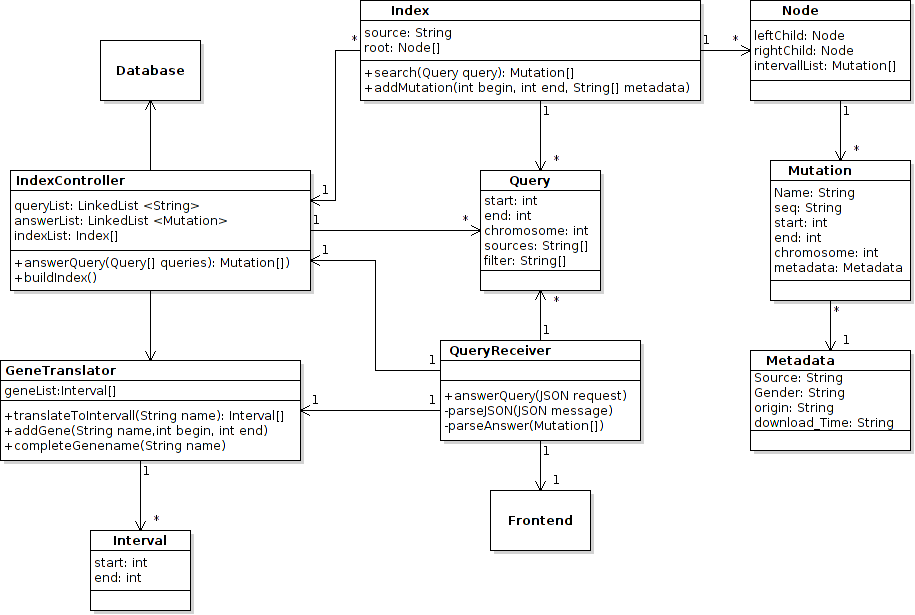
\includegraphics[width=1\textwidth]{middleware/Middleware_Class_final.png}
\caption{Schematischer Aufbau des Systems. Die Kommunikation mit dem Frontend findet über den QueryReceiver statt. Die Kommunikation mit der Datenbank übernimmt der IndexController. Die interne Kommunikation zwischen dem QueryReceiver, dem IndexController und den Indizes finden über Query-Objekte statt, die alle Informationen beinhalten, die für eine Suche benötigt wird. Der IndexController baut sowohl den Mutationsindex, als auch den GeneTranslator auf.}
\end{figure}
\begin{figure}[H]
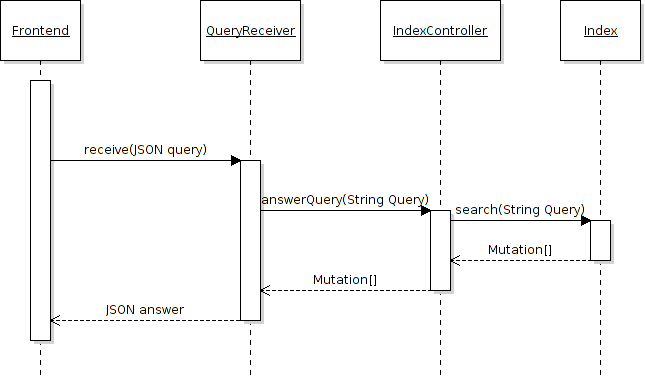
\includegraphics[width=1\textwidth]{middleware/intervall_seq.png}
\caption{Schematischer Ablauf einer Intervallanfrage. Der QueryReceiver erhält eine Anfrage, interpretiert diese und sendet eine Anfrage mit allen nötigen Informationen an den QueryHandler. Dieser ruft mit der Anfrage die Suchfunktionen der Teilindizes auf. Das Ergebnis wird zurückgereicht, ins Antwortformat gepackt und an das Frontend gesendet}
\end{figure}
\begin{figure}[H]
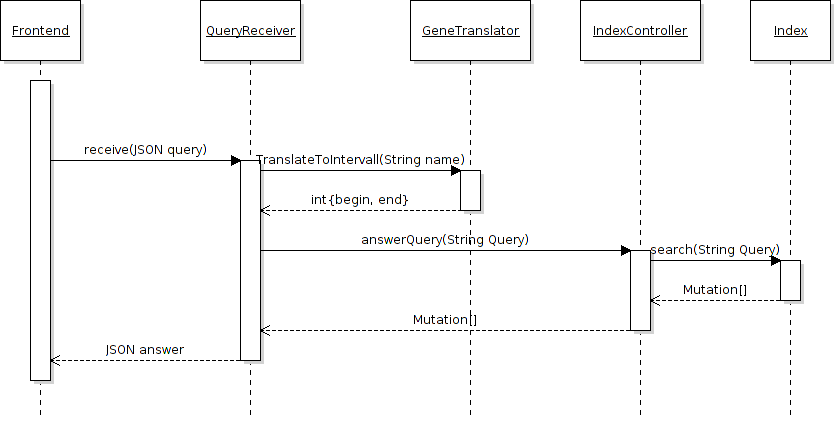
\includegraphics[width=1\textwidth]{middleware/namesearch_seq.png}
\caption{Schematischer Ablauf einer Gennamenanfrage. Nachdem der QueryReceiver die Nachricht erhalten hat schickt er den Gennamen an den GeneTranslator und erhält alle Intervalle, die dem Gen entsprechen. Mit dieser Information wird nun eine Query an den IndexController gestellt. Der weitere Ablauf ist identisch zu dem einer Intervallanfrage.}
\end{figure}
\begin{figure}[H]
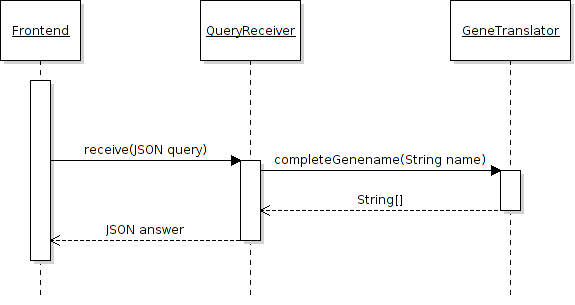
\includegraphics[width=1\textwidth]{middleware/prefix_seq.png}
\caption{Schematischer Ablauf einer Präfixsuche. Der QueryReceiver erhält eine Anfrage und leitet den Genpräfix in der Anfrage an den GeneTranslator weiter. Dieser gibt alle Gene zurück, die mit diesem Präfix beginnen. Die Antwort wird vom QueryReceiver in das Anfrageformat gepackt und an das Frontend gesendet.}
\end{figure}

\subsection{IndexController}
Der Index soll eine effiziente Suche nach Mutationen für das Frontend ermöglichen. Während des Programmstarts wird der Index aus der vorhandenen Datenbank aufgebaut und steht dann so lange zur Verfügung, bis das Programm beendet wird.
Im Index wird mit Intervallgrenzen gesucht und der Index gibt alle Intervalle zurück, die komplett innerhalb des angegebenen Intervalls liegen.\\
Der Index wird verteilt aufgebaut und liegt auf 4 virtuellen Maschinen verteilt. Die für den Index spezifizierten Funktionen sprechen immer einen Teilindex an. Der Aufruf der Funktionen wird über den IndexController erfolgen, der immer alle 4 Teilindizes ansprechen wird.
\subsubsection{Anforderungen}
Der IndexController ist für den Zugriff auf den Gesamtindex verantwortlich. Er nimmt Intervallanfragen entgegen und leitet diese an die Teilindizes weiter.
Die Teilergebnisse, die von den Indizes zurückgegeben werden, werden zusammengeführt und zurückgegeben.
Außerdem baut er zu Programmstart aus der bestehenden Datenbank heraus den Index auf.
\subsubsection{Funktionen}
\begin{itemize}
\item answerQuery(Query[] queries) returns Mutation[] answers\\
Die Funktion erhält eine Liste an Anfragen und gibt eine Liste aller Mutationen zurück, die den Anfrageforderungen entsprechen
\item buildIndex() returns void\\
Die Funktion baut den Index aus der Datenbank auf
\end{itemize}
\paragraph{answerQuery()}
Die Funktion erhält eine Liste an Query-Objekten. Ein Query-Objekt beinhaltet alle nötigen Information zu einer gegebenen Anfrage (gesuchtes Intervall, Quelle, Chromosom, Filterangaben)\\
Die Anfragen werden nebenläufig an die 4 Teilindizes weitergeleitet. Die einzelnen Teilergebnisse werden zusammengefasst und zurückgegeben.\\
\\
\begin{algorithm}
answerQuery()\\
\KwData{Query[] queries}
\KwResult{List of all matching Mutations for all queries}
Query[] queries\;
Index[] indices\;
Mutation[] answers=null\;
\ForAll{$q \in queries$}
{\ForAll{$i \in indices$}
{answers.add(i.search(q))\;}
}
return answers\;
\end{algorithm}


\paragraph{buildIndex()}
Die Funktion wird bei Programmstart ausgeführt und baut auf Basis der Datenbank die 4 Teilindizes auf. Der Zugriff auf die Datenbank erfolgt mithilfe des "JDBC41"-Treibers für "PostgreSQL". Es werden Anfragen der Form "SELECT * FROM Metadaten" und "SELECT * FROM Mutation" an die Datenbank gestellt, um mit den Ergebnissen die Indexstruktur zu befüllen. Wahrscheinlich werden die Anfragen noch geeignet aufgeteilt, da die Zwischenergebnisse sonst unter Umständen zu groß für den Hauptspeicher wären.\\
Für jede Mutation wird zufällig entschieden in welchen Index sie eingefügt wird.\\
Nachdem der Gesamtindex aufgebaut wird, wird der GeneTranslator aus der Datenbank "RefSeq" aufgebaut.
\begin{algorithm}
buildIndex()\\
\KwData{--}
\KwResult{A built index}
connect to mutation\_database\;
ResultSet rs = executeQuery(query1)\;
GeneTranslator j\;
\ForAll{elements e $\in$ rs}
{choose sub index i to insert into\;
i.addMutation()\;}
connect to genename\_database\;
rs = executeQuery(query2)\;
\ForAll{elements e $\in$ rs}
{j.insert(e)\;}
return\;
\end{algorithm}
\newpage

\subsection{Index}
\subsubsection{Anforderungen}
Der Index soll eine effiziente Suche nach Mutationen ermöglichen. Dabei gibt es die Möglichkeiten direkt nach einem Intervall zu suchen oder aber nach allen Mutationen zu suchen, die auf einem bestimmten Gen liegen. Während des Programmstarts wird der Index aus der vorhandenen Datenbank aufgebaut und steht dann so lange zur Verfügung, bis das Programm beendet wird.\\
Im Index wird mit Intervallgrenzen gesucht und der Index gibt alle Intervalle zurück, die sich in irgendeinem Punkt mit dem gesuchten Intervall überschneiden.\\
Der Index wird verteilt aufgebaut und teilt sich auf 4 virtuellen Maschinen auf. Die für den Index spezifizierten Funktionen sprechen immer einen der 4 Teilindizes an. Der Aufruf der Funktionen wird über den IndexController erfolgen, der immer alle 4 Teilindizes ansprechen wird.

\subsubsection{Datenstruktur für den Index}
Die dem Index zugrundeliegende Datenstruktur ist ein Intervallbaum. Dieser ermöglicht effizientes Suchen nach und Einfügen von Intervallen.\\
Hierfür wird die frei zugängliche Bibliothek "IntervalST.java" der Universität Princeton als Grundgerüst verwendet. Die vorgenommenen Änderungen belaufen sich hauptsächlich auf eine Anpassung der verwendeten Datenstrukturen, eine Erweiterung der Suchfunktion um Filter und einen geeigneten Umgang mit Duplikaten (mehrere Mutationen auf demselben Intervall). Außerdem können einige für uns unnötige Funktionen entfernt werden. Die Funktionen addMutation() und search() dienen als Interface zu den in der Bibliothek definierten Funktionen, die Elemente einfügen und suchen\\
Das Suchergebnis wird nach den bei der Anfrage spezifizierten Filtern gefiltert. Bei n Intervallen und einer Such-Ergebnisliste der Größe m ergibt sich ein Komplexität von $\mathcal{O}$(log n + m)\\
\subsubsection{Funktionen}
\begin{itemize}
\item addMutation(Mutation mutation)returns void\\
Die Funktion erhält eine Mutation, die eingefügt werden soll
\item search(Query query)returns Mutation[]\\
Die Funktion erhält eine Anfrage und gibt alle Mutation zurück, die den Anfrageanforderungen entsprechen
\end{itemize}
\newpage
\paragraph{addMutation()}
Die Funktion erhält eine Mutation als Parameter und fügt diese in Indexstruktur ein.
\begin{algorithm}
addMutation()\\
\KwData{Mutation input}
\KwResult{input added to index}
IntervalTree i\;
insert input into i\;
return\;
\end{algorithm}
\paragraph{search()}
Die Funktion erhält eine Anfrage nach dessen Kriterien nach Mutationen gesucht werden soll und einen Knoten des Baumes (zu Beginn der Wurzelknoten). Es werden alle Mutationen gesucht, die komplett oder teilweise innerhalb der Intervallgrenzen liegen. Für alle Mutationen auf die dies zutrifft wird geprüft, ob sie den Filtern entsprechen nach denen gesucht wird. Alle Elemente, die die Filtereinschränkung erfüllen werden zurückgegeben.
\begin{algorithm}
search()\\
\KwData{Query input, Node current}
\KwResult{List of all matching mutations}
IntervalTree i\;
Mutation[] answer\_list\;
{\eIf{current node matches searched interval}
{add mutation to answer\_list if it corresponds to specified filters\;}
{continue search in subtrees\;}}
return answer\_list\;
\end{algorithm}
\newpage

\subsection{GeneTranslator}
\subsubsection{Anforderungen}
Der GeneTranslator wird aufgerufen, falls es sich bei der Anfrage um eine Präfixsuche oder eine Gennamensuche handelt. Die Komponente beinhaltet eine Datenstruktur, die alle im System vorhandenen Gennamen und ihre Intervallbereiche beinhaltet.\\
Die Komponente ermöglicht eine effiziente Suche nach Gen-Präfixen und nach Gennamen um die zugehörigen Intervalle zu erfragen.\\
Als interne Datenstruktur wird ein PatriciaTrie genutzt. Dieser ist in der frei zugänglichen Bibliothek "Apache Commons" vorhanden und wird für diese Implementation genutzt.

\subsubsection{Funktionen}
\begin{itemize}
\item translateToInterval(String name) returns Intervall[]\\
Die Funktion erhält einen Gennamen, nach dem gesucht wird und gibt eine Liste von Intervallobjekten zurück, die den Start-und den Endpunkt aller Vorkommen des Gens beinhalten
\item addGene(String name, int begin, int end) returns void\\
Die Funktion erhält einen Gennamen und die Intervallgrenzen des Gens und fügt diese in die zur Suche benötigten Datenstruktur ein
\item completeGenename(String name) returns String[]\\
Die Funktion erhält einen Präfix eines Gennamens und gibt alle Gennamen zurück, die mit diesem Präfix beginnen
\end{itemize}
\paragraph{translateToInterval()}
Diese Funktion wird aufgerufen, falls eine Gensuche angefragt wird. Sie überstetzt das gesuchte Gen in die zugehörigen Intervalle um eine Intervallsuche aus der Anfrage zu machen, die vom Index bearbeitet werden kann.

\paragraph{addGene()}
Die Funktion fügt der internen Datenstruktur ein Gen und die zugehörigen Intervalle hinzu. Sollte sich das Gen bereits in der Struktur befinden, so wird überprüft, ob eines der vorhandenen Intervalle für diesen Gen komplett im neu hinzugefügten befindet. Ist dies der Fall, so wird das alte Intervall durch das neue ersetzt. Andernfalls wird das neue Intervall an die Liste der Intervalle für dieses Gen zugefügt. Sollten die Intervalle eines Gens komplett denen eines anderen Gens entsprechen, so kann davon ausgegangen werden, dass diese synonyme Bezeichnungen für das gleiche Gen sind. Da die Intervalle bereits gleich sind werden Synonyme implizit abgefangen.

\paragraph{completeGenename()}
Die Funktion gibt alle Gennamen zurück, die mit dem gesuchten Präfix beginnen\\
\newpage

\subsection{QueryReceiver}
\subsubsection{Anforderungen}
Der QueryReceiver bildet die direkte Schnittstelle zum Frontend. Alle Anfragen, die der Nutzer eingibt werden als JSON-File an ihn gesendet und Antworten werden von ihm an das Frontend zurückgegeben. Die Komponente überprüft für alle eingehenden Anfragen um was für eine Anfrage-Art es sich handelt und leitet sie an die zuständigen Teilkomponenten weiter.\\
Für die einzelnen JSON-Formate siehe Abschnitt Schnittstelle GUI-Middleware\\

\subsubsection{Funktionen}
\begin{itemize}
\item answerQuery(JSON request) returns JSON answer\\
Die Funktion erhält eine Anfrage im JSON-Format und gibt eine Antwort im JSON-Format zurück
\end{itemize}
\paragraph{answerQuery()}
Alle Nutzer-Anfragen werden an diese Funktion gesendet. Sie überprüft anhand des Aufbaus der JSON-Anfrage, um was für eine Anfrageart es sich handelt.\\ Bei der Intervallsuche wird die JSON-Anfrage in ein Query-Objekt umgewandelt und an den IndexController weitergeleitet. Bei der Gennamensuche wird zuerst im GeneTranslator nach dem zum Gen gehörigen Intervall gesucht und mit dieser Information und den Filterangaben des Nutzers ein Query-Objekt erstellt, dass dem IndexController übergeben wird. Handelt es sich um eine Präfixsuche wird im Genetranslator nach Gennamen gesucht, die mit dem Präfix beginnen. Die Antworten der jeweiligen Anfragen werden in das zum Anfragetyp gehörende JSON-Antwortformat verpackt und an das Frontend zurückgesendet.\\

\newpage
\section{Stresstest}
Der Stresstest hat zum Ziel herauszufinden, wie lange die durchschnittliche Query-Laufzeit ist.\\
Ziel des Systems ist es eine Laufzeit von unter einer Sekunde zu erreichen.\\
Um dies zu überprüfen werden zufällig je 50 korrekte Anfragen der gleichen Art (Intervallsuche, Gennamenssuche, Präfixsuche) an das System gestellt und die Antwortzeiten gemessen. Diese dürfen alle nicht länger als eine Sekunde zur Antwort brauchen.\\
Hierfür wird ein Testprogramm geschrieben, dass Anfragen im korrekten Format stellt und die Antwortzeiten automatisch auswertet. Die Anfragen werden zufällig generiert.

\newpage
\subsection{Unit-Tests}
\subsubsection{QueryReceiver}
\textbf{Testfall 1 - erfolgreiche Intervallanfrage ohne Metadaten}
\begin{verbatim}
  Eingabe
{
  "source": The Cancer Atlas,\usepackage[utf8]{inputenc}
  "chromosome": 3,
  "position": {"from": 100, "to": 200},
  "zoom": 1,
  "subindex": ,
  "hasDetail": (false)
}

  Ausgabe
{
  {
    "source:" The Cancer Atlas,
    "chromosome": 3,
    "position": {"from": 100, "to": 200},
    "details": { "refseq": ,
                "mutations": [{ "name": ,
                                "position": {"from": , "to": },
                                "metadata":
                              },]},
    "graph": {
              { "subintervall": Anzahl der Subintervalle,
                "counts": Anzahl der Ergebnisse
              }
            }
  }
}
\end{verbatim}
\textbf{Testfall 2 - erfolgreiche Intervallanfrage mit Metadaten}
\begin{verbatim}
  Eingabe
{
  "source": The Cancer Atlas,
  "chromosome": 3,
  "position": {"from": 100, "to": 200},
  "zoom": 1,
  "subindex": ,
  "hasDetail": (true)
}

  Ausgabe
{
  {
    "source:" The Cancer Atlas,
    "chromosome": 3,
    "position": {"from": 100, "to": 200},
    "details": { "refseq": Referenzsequenz,
                "mutations": [{Mutation1},{Mutation2},...]},
    "graph": {
              { "subintervall": ,
                "counts":
              }
            }
  }
}
\end{verbatim}
\textbf{Testfall 3 - Intervallanfrage mit leerer Antwortmenge}
\begin{verbatim}
  Eingabe
{
  "source": The Cancer Atlas,
  "chromosome": 3,
  "position": {"from": 100, "to": 200},
  "zoom": 1,
  "subindex": ,
  "hasDetail": (true)
}

  Ausgabe
{
  {
    "source:" The Cancer Atlas,
    "chromosome": 3,
    "position": {"from": 100, "to": 200},
    "details": { "refseq": ,
                "mutations": ...},
    "graph": {
              { "subintervall": ,
                "counts":
              }
            }
  }
}
\end{verbatim}
\newpage\hfill\\
\textbf{Testfall 4 - erfolgreiche Namensanfrage}
\begin{verbatim}
  Eingabe
{
  "source": The Cancer Atlas,
  "chromosome": 3,
  "search": "Gen im Cancer Atlas"
}

  Ausgabe
{
  "source": The Cancer Atlas,
  "chromosome": 3,
  "search": "Gen im Cancer Atlas",
  "position": {"from": Startposition, "to": Endposition}
}
\end{verbatim}
\textbf{Testfall 5 - Namensanfrage mit leerer Antwortmenge}
\begin{verbatim}
  Eingabe
{
  "source": The Cancer Atlas,
  "chromosome": 3,
  "search": "Gen, dass nicht im Cancer Atlas ist"
}

  Ausgabe
{
  "source": The Cancer Atlas,
  "chromosome": 3,
  "search": "Gen im Cancer Atlas",
  "position": " "
}
\end{verbatim}
\textbf{Testfall 6 - fehlerhafte Anfrage}
\begin{verbatim}
  Eingabe
{
  "source": ""
}

  Ausgabe
{
  "answer": "unknown format"
}
\end{verbatim}
\newpage
\subsubsection{IndexController}
Um den IndexController zu testen wird ein Testprogramm genutzt, dass Anfragen stellt und das Ergebnis mit vorher manuell abgefragten Ergebnissen abgleicht:
\begin{verbatim}
import static org.junit.Assert.*;
import java.io.*;
import java.util.*;

public class IndexTest {
	public static void main(String[] args) throws IOException  {
		QueryHandler x_QH = new QueryHandler();
		File x_File = new File("./testQueries.txt");
		FileReader x_FR = new FileReader(x_File);
      	BufferedReader x_BR = new BufferedReader(x_FR);
      	String query[] = new String[1];
      	String answer = "";
      	String result = "";
      	Set<IntervalST.Node> x_Result = new HashSet<IntervalST.Node>();
      	while ((query[0] = x_BR.readLine()) != null) {
      		result = "";
      		if ((answer = x_BR.readLine()) != null) {
      			x_Result = x_QH.answerQuery(query);
      			for (IntervalST.Node x_Node : x_Result) {
      				result = result + x_Node.i_MutationID;
    			}
    			assertEquals(answer, result);		//compares expected answer and the result of the query
      		} else {
      			break;
      		}
      	}
	}
}
\end{verbatim}
Die Datei mit den Testdaten sieht folgendermaßen aus:
\begin{verbatim}
7775,7779
0
6463,6465
13
24141,24146
5
5323,5327
11
32445,32448
21
4535,4535
2
22550,22600
1
9700,10000
19
44000,45000
15
50000,60000
7
\end{verbatim}
\subsubsection{GeneTranslator}
\textbf{Testfall 1 - addGene - Einfügen in Datenstruktur}\\
Eingabe: Testgen, 350, 500\\
Ausgabe: Dass Gen sollte in den Baum eingefügt sein und per searchForGene() findbar sein\\
\\
\textbf{Testfall 2 - addGene - Doppeltes Einfügen in Datenstruktur}\\
Eingabe: Testgen, 350, 500\\
		 Testgen, 350, 500\\
Ausgabe: Dass Gen sollte nur einmal in die Datenstruktur eingefügt werden. Ausgabe, dass das Gen bereits in der Struktur vorhanden ist.\\
\\
\textbf{Testfall 3 - addGene - Aufruf ohne Parameter}\\
Eingabe: [...]\\
Ausgabe: Fehlermeldung über  parameterlosen Aufruf\\
\\
\textbf{Testfall 4 - tranlateToIntervall - erfolgreiche Suche}\\
Eingabe: Testgen (befindet sich bereits in Datenstruktur)\\
Ausgabe: 350, 500\\
\\
\textbf{Testfall 5 - tranlateToIntervall - erfolglose Suche}\\
Eingabe: Testgen2 (befindet sich nich in Datenstruktur)\\
Ausgabe: Fehlermeldung über erfolglose Suche\\
\\
\textbf{Testfall 6 - tranlateToIntervall - Aufruf ohne Parameter}\\
Eingabe: [...]\\
Ausgabe: Fehlermeldung über Parameterlosen Aufruf\\
\\
\textbf{Testfall 7 - completeGeneName - erfolgreiche Suche mit einem Ergebnis}\\
Eingabe: Test (Testgen1 befindet sich bereits in Datenstruktur)\\
Ausgabe: Testgen1\\
\\
\textbf{Testfall 8 - completeGeneName - erfolgreiche Suche mit mehreren Ergebnissen}\\
Eingabe: Test (Testgen1 und Testgen2 befinden sich bereits in Datenstruktur)\\
Ausgabe: Testgen1, Testgen2\\
\\
\textbf{Testfall 9 - completeGeneName - erfolglose Suche}\\
Eingabe: Test (Es befindet sich kein Gen mit Präfix Test in der Datenstruktur)\\
Ausgabe: Fehlermeldung über erfolglose Suche
\subsubsection{Intervallbaum}
\textbf{1. Intervalle einfügen:}\\
Das Intervall muss im Baum an der richtigen Stelle eingefügt werden und der Baum muss gegebenenfalls neu balanciert werden (z.B. wie ein AVL-Baum).\\\\
Bsp.: Einfügen des Intervalls [12,15]
\begin{figure}[H]
 \centering
	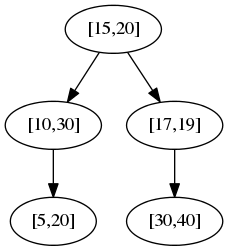
\includegraphics[width=0.2\textwidth]{middleware/Testfaelle/1.png}
	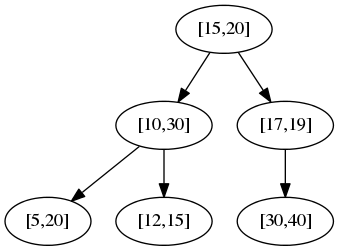
\includegraphics[width=0.3\textwidth]{middleware/Testfaelle/2.png}
\end{figure}
\textbf{2. Intervall mit Startpunkt $>$ Endpunkt einfügen:}\\
Wenn ein Intervall (S,E) mit S$>$E eingefügt wird, dann sollte unser Programm eine Fehlermeldung ausgeben und darauf hinweisen, dass die Grenzen für das Intervall nicht korrekt sind.\\\\
Bsp.: Einfügen des Intervalls [20,10] in einen beliebigen Baum.\\\\
\textbf{3. Intervall mit Start- bzw. Endpunkt außerhalb des betrachteten Zahlenbereichs:}\\
Wenn ein Intervall in dem Baum eingefügt werden soll, das teilweise oder vollständig außerhalb unseres Zahlenbereichs liegt (Länge des Genoms), dann muss es eine Fehlermeldung geben, die dem Nutzer mitteilt, dass der gültige Zahlenbereich überschritten wurde.\\\\
Bsp.: Einfügen des Intervalls [-5,7] in einen beliebigen Baum.\newpage\hfill\\
\textbf{4. Schon vorhandenes Intervall einfügen:}\\
Duplikate sollen von unserem Baum nicht gespeichert werden, d.h. es wird kein neuer Knoten hinzugefügt, sondern die Informationen (bei uns also Pointer auf Dateien) des neuen Knotens müssen im bereits vorhandenen Knoten mitgespeichert werden.\\\\
Bsp.: Einfügen des Intervalls [15,20] in den folgenden Baum\\\\
\includepicture[width=0.2\textwidth]{middleware/Testfaelle/1.png}{ }
\textbf{5. Suche nach vorhandenem Intervall:}\\
Bei der Suche sollen alle Intervalle ausgegeben werden, die das gesuchte Intervall in irgendeinem Punkt überlappen.\\\\
Bsp.: Suche im folgenden Baum\\\\
\includepicture[width=0.3\textwidth]{middleware/Testfaelle/2.png}{ }
Suche [4,5] $\Rightarrow$ gib [5,20] aus\\
Suche [25,35] $\Rightarrow$ gib [10,30] und [30,40] aus\\
Suche [20,20] $\Rightarrow$ gib [15,20] und [5,20] aus
\subsection{Stresstests}
Der Stresstest hat zum Ziel herauszufinden, wie lange die durchschnittliche Query-Laufzeit ist.\\
Ziel des Systems ist es eine Laufzeit von unter einer Sekunde zu erreichen.\\
Um dies zu überprüfen werden zufällig je 50 korrekte Anfragen der gleichen Art (Intervallsuche, Gennamenssuche, Präfixsuche) an das System gestellt und die Antwortzeiten gemessen. Diese dürfen alle nicht länger als eine Sekunde zur Antwort brauchen.\\
Hierfür wird ein Testprogramm geschrieben, dass Anfragen im korrekten Format stellt und die Antwortzeiten automatisch auswertet. Die Anfragen werden zufällig generiert.


\newpage

\section{Schnittstellenspezifikation: Middleware - Frontend}
Bei der Kommunikation zwischen Middleware und Forntend ist ein Austausch von JSON über die HTTP-Methode GET vorgesehen.
An die Middleware werden folgende Informationen geschickt:
\\
\textit{Quellen; Chromosom; Position; Suche; Präfix-Flag; Zoomstufe; Anzahl der Subintervalle; HasDetail-Flag}.\\
Von der Middleware werden bei bestimmten Flags, folgende Daten erwartet:
\\
Wenn \textit{IsPräfix-Flag} = \texttt{true}: Array aller Präfixe\\
Wenn \textit{IsPräfix-Flag} = \texttt{false}: Name und Position der Suche\\[1em]
Wenn \textit{HasDetail-Flag} = \texttt{true}: RefSeq + Mutationen mit MetaDaten\\
Wenn \textit{HasDetail-Flag} = \texttt{false}: aggregierte Mutationen (durch Zoomstufe+Anzahl der \textit{Subintervalle})

\subsubsection{Suchanfrage JSON}
GUI $\Rightarrow$ Middleware
\begin{lstlisting}[language=c,
commentstyle=\fontsize{12}{14.4}\ttfamily,
basicstyle=\ttfamily\fontsize{10}{12}\selectfont, showstringspaces=false]
{
  "source": ["src1", "src2", ...],
  "chromosome": int x,
  "search": String a
  "isPrefix": (true|false)
}
\end{lstlisting}
GUI $\Leftarrow$ Middleware
\begin{lstlisting}[language=c,
commentstyle=\fontsize{12}{14.4}\ttfamily,
basicstyle=\ttfamily\fontsize{10}{12}\selectfont, showstringspaces=false]
{
  "source": ["src1", "src2", ...],
  "chromosome": int x,
  "search": String a,
  "prefix": ["String a", "String b", ...],
  "position": {"from": int x, "to": int y}
}
\end{lstlisting}
\paragraph{Bemerkung} Wenn das \textit{isPrefix} den Wert \texttt{'true'} besitzt, wird \texttt{"prefix"} befüllt mit einem Array aller möglichen Präfixe.\\
Wenn das \textit{isPrefix} den Wert \texttt{'false'} besitzt, wird \texttt{"prefix"} nicht befüllt, aber \texttt{"'search"} und \texttt{"position"} werden dann befüllt.
\newpage

\subsubsection{Intervallanfrage JSON}
GUI $\Rightarrow$ Middleware
\begin{lstlisting}[language=c,
commentstyle=\fontsize{12}{14.4}\selectfont,
basicstyle=\ttfamily\fontsize{10}{12}\selectfont, showstringspaces=false]
{
  "source": String s,
  "chromosome": int x,
  "position": {"from": int x, "to": int y},
  "zoom": int y,
  "subindex": int z,
  "hasDetail": (true|false)
}
\end{lstlisting}
GUI $\Leftarrow$ Middleware (pro Quelle)
\begin{lstlisting}[language=c,
commentstyle=\fontsize{12}{14.4}\selectfont,
basicstyle=\ttfamily\fontsize{10}{12}\selectfont, showstringspaces=false]
{
  {
    "source:" String s,
    "chromosome": int x,
    "position": {"from": int x, "to": int y},
    "details": { "refseq": String b,
                "mutations": [{ "name": String s,
                                "position": {"from": int x, "to": int y},
                                "metadata": {...}
                              },{...},...]},
    "graph": {
              { "subintervall": int x,
                "counts": int y
              },
              {...}
            }
  }
}
\end{lstlisting}
\paragraph{Bemerkung} Wenn das \textit{HasDetail-Flag} \texttt{'true'} ist, dann wird \texttt{"detail"} befüllt und \texttt{"graph"} bleibt leer.\\
Wenn das \textit{HasDetail-Flag} \texttt{'false'} ist, dann wird \texttt{"graph"} befüllt und \texttt{"detail"} bleibt leer.\\
Mit \texttt{"'subindex"} ist die Anzahl der \textit{Subintervalle} gemeint. Als \textit{Subintervalle} werden kleine Bereiche des Intervalls bezeichnet. Diese werden dazu verwendet um einen Graphen detalierter darzustellen.
\newpage
\subsection{Beispiel der Kommunikation mit JSON}
\paragraph{Suchanfrage} Es wird eine Suchanfrage des Users getätigt. Die \textit{Suche} wird mit dem Wert \textit{"FOXP2"} befüllt.\\
\newline
GUI $\Rightarrow$ Middleware
\begin{lstlisting}[language=c,
commentstyle=\fontsize{12}{14.4}\selectfont,
basicstyle=\ttfamily\fontsize{10}{12}\selectfont, showstringspaces=false]
{
  "source": ,
  "chromosome": ,
  "search": "FOXP2"
  "isPrefix": false
}
\end{lstlisting}
GUI $\Leftarrow$ Middleware
\begin{lstlisting}[language=c,
commentstyle=\fontsize{12}{14.4}\selectfont,
basicstyle=\ttfamily\fontsize{10}{12}\selectfont, showstringspaces=false]
{
  "chromosome": 7,
  "search": "FOXP2",
  "prefix": [],
  "position": {"from": 114086310, "to": 114693772}
}
\end{lstlisting}
Darauf folgt eine Intervallanfrage mit der \textit{Zoomstufe} von \texttt{'1,000,000bp'} und der Anzahl der Subintervalle von \texttt{'200'}.\\
\newline
GUI $\Rightarrow$ Middleware
\begin{lstlisting}[language=c,
commentstyle=\fontsize{12}{14.4}\selectfont,
basicstyle=\ttfamily\fontsize{10}{12}\selectfont, showstringspaces=false]
{
  "source": "Source 1",
  "chromosome": 7,
  "position": {"from": 114086310, "to": 114693772},
  "zoom": 1,000,000,
  "subindex": 200,
  "hasDetail": false
}
\end{lstlisting}
GUI $\Leftarrow$ Middleware
\begin{lstlisting}[language=c,
commentstyle=\fontsize{12}{14.4}\selectfont,
basicstyle=\ttfamily\fontsize{10}{12}\selectfont, showstringspaces=false]
{
  {
    "source:" "Source 1",
    "chromosome": 7,
    "position": {"from": 114086310, "to": 114693772},
    "details": {},
    "graph": {
              { "subintervall": 114091310,
                "counts": 233
              },
              {
                "subintervall": 114096310,
                "counts": 122
              },
              {
                "subintervall": 114101310,
                "counts": 89
              },
              {
                "subintervall": 114106310,
                "counts": 234
              },
              {...},
              ...
            }
  }
}
\end{lstlisting}

\paragraph{Intervallsuche} Der User gibt ein \textit{Intervall} an und möchte sich in der niedrigsten \textit{Zoomstufe} die Details anschauen.\\
\newline
GUI $\Rightarrow$ Middleware
\begin{lstlisting}[language=c,
commentstyle=\fontsize{12}{14.4}\selectfont,
basicstyle=\ttfamily\fontsize{10}{12}\selectfont]
{
  "source": "Source 1",
  "chromosome": 14,
  "position": {"from": 5465, "to": 5665},
  "zoom": 200,
  "subindex": 0,
  "hasDetail": true
}
\end{lstlisting}
GUI $\Leftarrow$ Middleware
\begin{lstlisting}[language=c,
commentstyle=\fontsize{12}{14.4}\selectfont,
basicstyle=\ttfamily\fontsize{10}{12}\selectfont,showstringspaces=false]
{
  {
    "source:" Source 1,
    "chromosome": 14,
    "position": {"from": 5465, "to": 5665},
    "details": { "refseq": "CCCTGAGAAAGACGCCCTGAGCGGGTAACGTCAACTGTCG
			    TGGGATTGGAAGAACTTGGTGGGGTTCCACATATCATGAT
                            CACGTAGAACACAATAAAGAAAATCTCCGGAGCGTGAATT
                            AAACTGAACTGACTCTTGTCAGTGTCTCGCTTACCACGTC
                            AAGGAAGTCAATGATGCCCTAATCTGGATAGCTTTGTCAT",
                "mutations": 
                [{ "name": "RS12334",
                                "position": {"from": 5480, "to": 5498},
                                "metadata": {"sequence": "TCGGTATTCTACGTCTGC"}
                              },
                 { "name": "RBDDFG23",
                                "position": {"from": 5560, "to": 5567},
                                "metadata": {"sequence": "GGGCACT"}
                              }
                 { "name": "RS12334",
                                "position": {"from": 5599, "to": 5610},
                                "metadata": {"sequence": "TGACGAGATCG"}
                              }
                 { "name": "RS12334",
                                "position": {"from": 5650, "to": 5655},
                                "metadata": {"sequence": "CGACC"}
                              }]
              },
    "graph": {}
  }
}
\end{lstlisting}

\newpage

\section{Frontend}
\subsection{Mock-Ups der Benutzerschnittstelle}
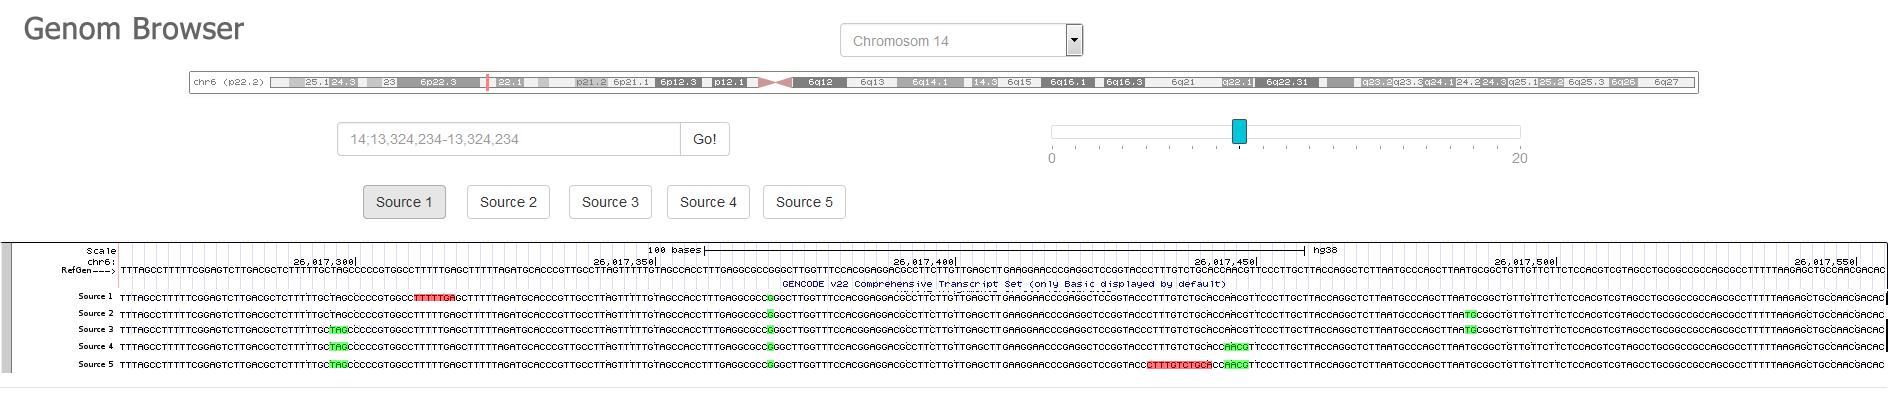
\includegraphics[width=\textwidth]{gui/gb_mockup_detail_view.png}
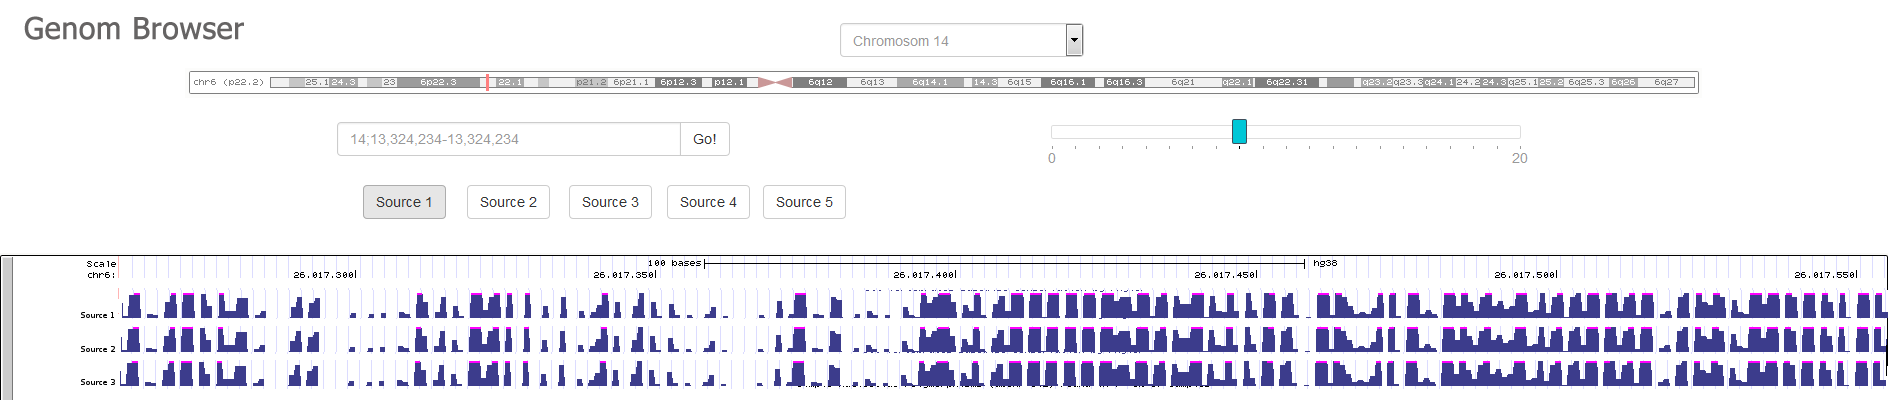
\includegraphics[width=\textwidth]{gui/gb_mockup_index_view.png}
\subsection{Klassen-Diagramm}
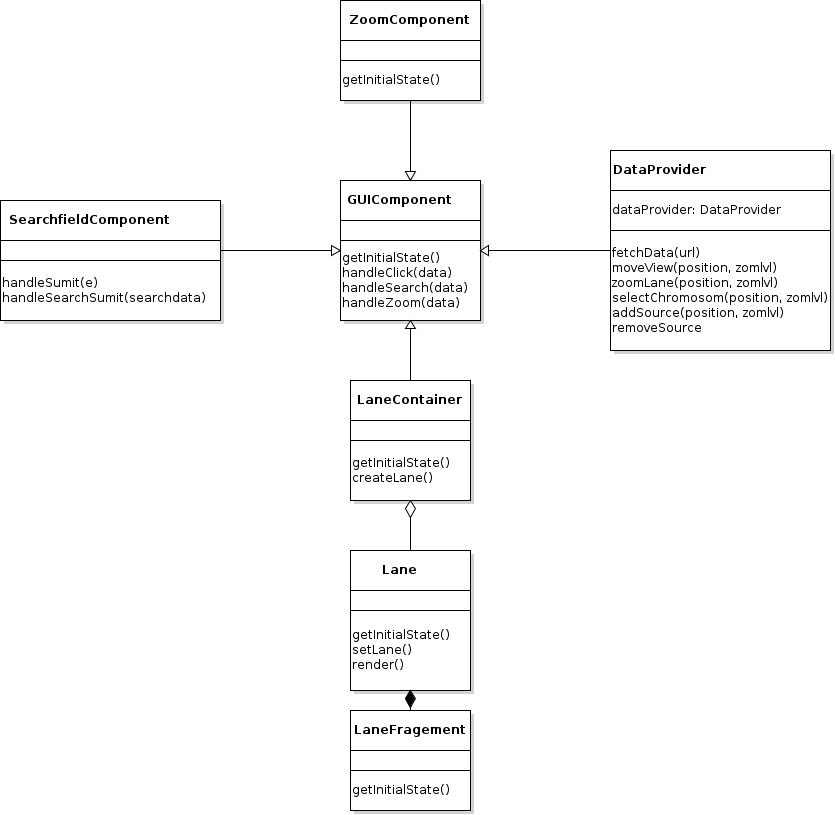
\includegraphics[width=\textwidth]{gui/gui-klassendiagramm.png}
\subsection{Sequenzdiagramm}
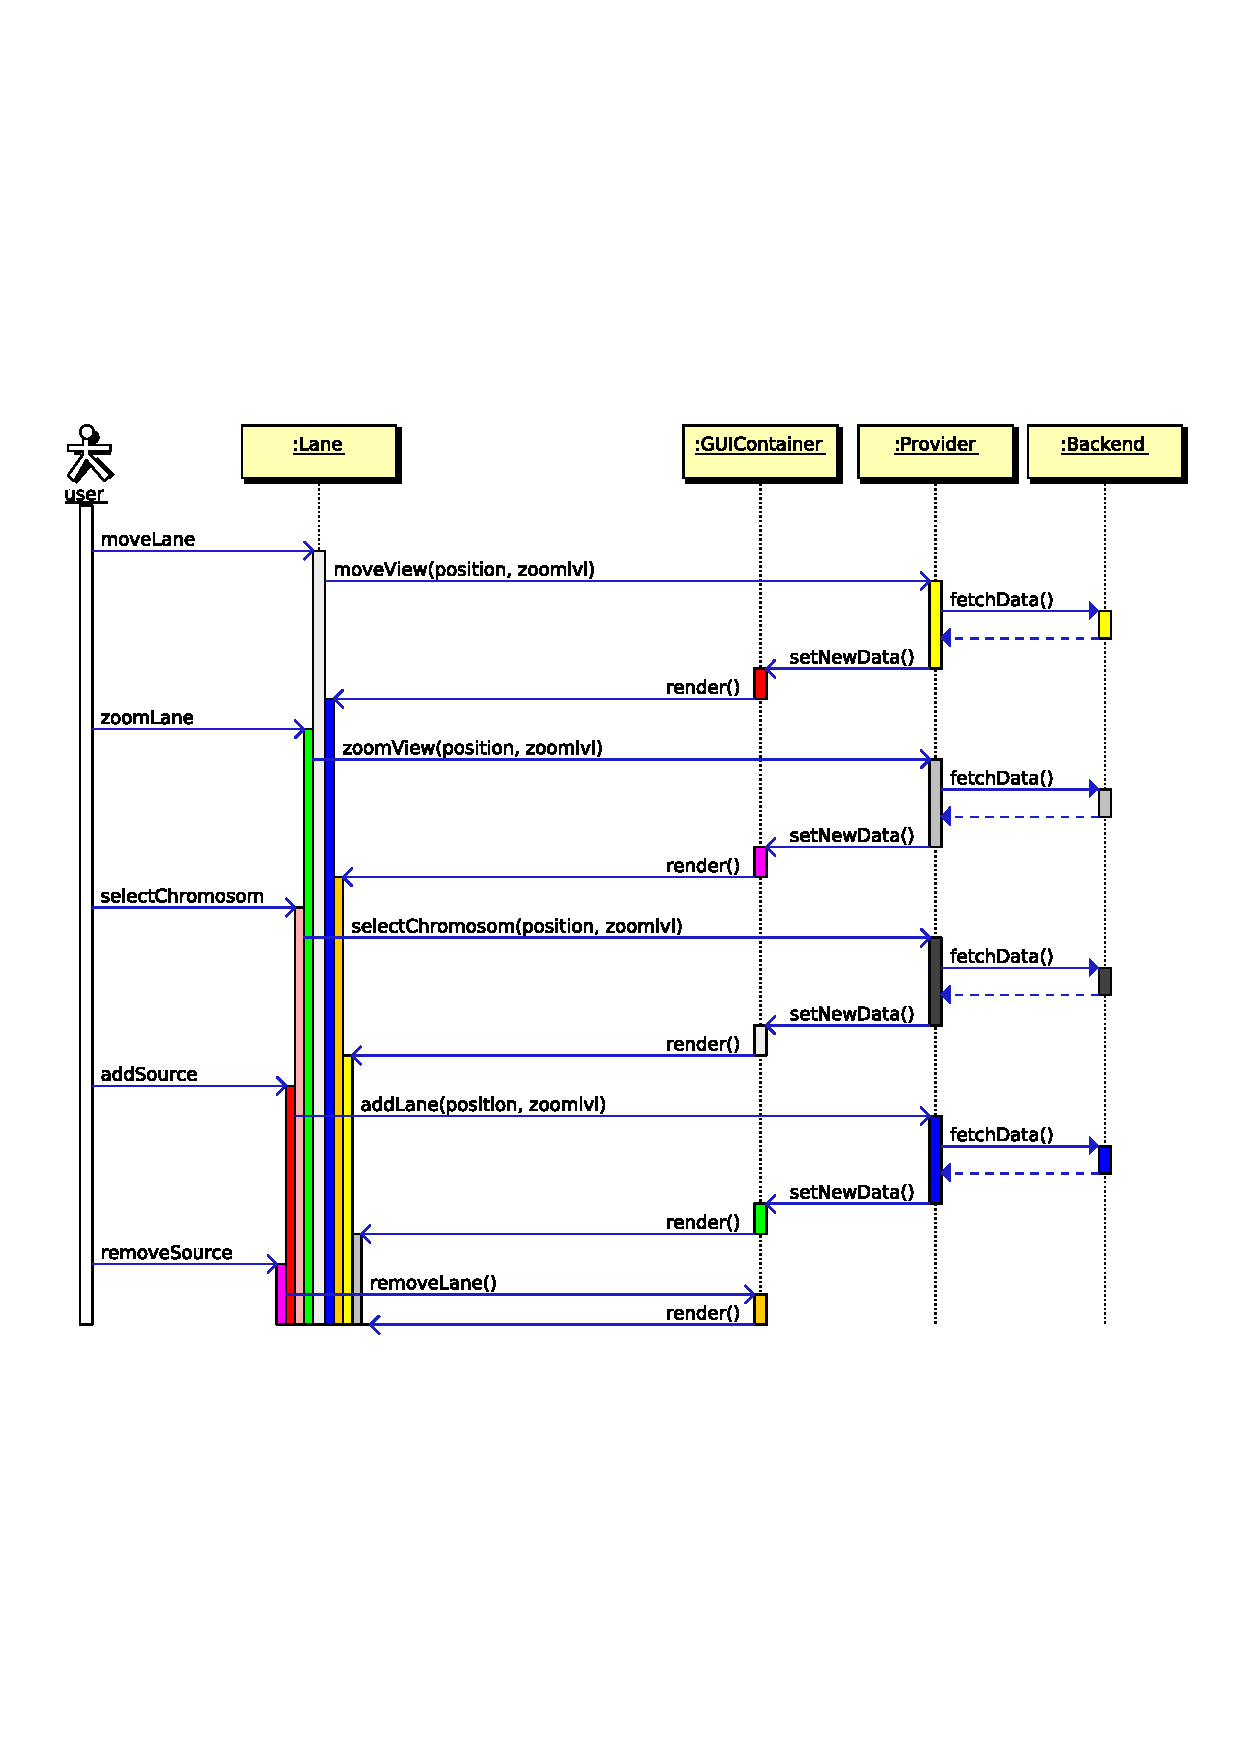
\includegraphics[width=\textwidth]{gui/GUI_Sequenzdiagramm.pdf}
\subsection{Use Cases}
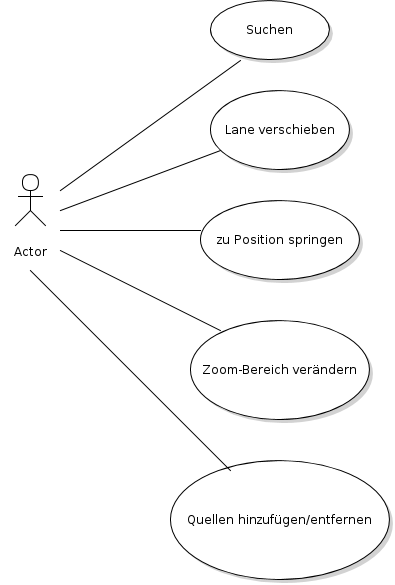
\includegraphics[width=\textwidth]{gui/gui-usecasediagramm.png}
\subsection{Unit-Tests}
\subsubsection{Suchfunktion}
\begin{enumerate}
	\item Wenn ich als Nutzer eine leere Suche starte, dann möchte ich eine entsprechende Fehlermeldung angezeigt bekommen.
	\item Wenn ich eine Suche mit falscher Eingabe starte, dann möchte ich eine entsprechende Fehlermeldung angezeigt bekommen.
	\item Wenn ich als Nutzer nach einem gültigen Intervall suche, dann wird automatisch die Zoomstufe auf dieses Intervall angepasst.
	\item Wenn ich als Nutzer nach einem vorhandenem Gene suche, dann wird automatisch die Zoomstufe auf dieses Intervall angepasst.
\end{enumerate}


\subsubsection{Quellen-Button}
\begin{enumerate}
	\item Wenn ich als Nutzer auf einen "Quellen"-Button drücke, dann wird mir die entsprechende Quelle zusätzlich zu den bereits dargestellten Quellen, angezeigt.
	\item Wenn ich als Nutzer auf den "Quellen"-Button einer bereits angezeigten Quelle drücke, wird die entsprechende Quelle nicht mehr angezeigt.
\end{enumerate}

\subsubsection{Quellen-Scroller}
\begin{enumerate}
	\item Als Nutzer kann ich mich über horizontales Scrolling synchron durch die Quellen bewegen.
\end{enumerate}

\subsubsection{Zoom-slider}
\begin{enumerate}
	\item Wenn ich die Zoomstufe über den Slider ändere, dann werden die Quellen entsprechend der eingestellten Stufe dargestellt.
	\item Wenn ich als Nutzer die feinste Zoomstufe einstelle, dann werden mir die Basenpaare angezeigt.
	\item Wenn ich als Nutzer eine andere Zoomstufe einstelle, dann werden mir aggregierten Daten angezeigt.
\end{enumerate}

\subsubsection{Chromosom-Auswahl}
\begin{enumerate}
	\item Als Nutzer kann ich über ein Dropdown aus einer Vorauswahl von Chromosomen auswählen.
	\item Wenn ich als Nutzer ein Chromosom auswähle, dann wird die Quellen-Anzeige automatisch entsprechend des ausgewählten Chromosoms aktualisiert.
	\item Wenn ich als Nutzer das bereits ausgewählte Chromosom erneut auswählen, dann passiert nichts.
\end{enumerate}

\subsubsection{Allgemein}
\begin{enumerate}
	\item Wenn ich als Nutzer auf eine Anfrage warten muss, wird mir dies durch einen Loading-Spinner signalisiert.	
\end{enumerate}
\newpage

%\section{Integrationstest}
%\subsection{Ablauf der Integrationstests}


\end{document}